\documentclass[conference]{IEEEtran}
\IEEEoverridecommandlockouts
\usepackage{cite}
\usepackage{amsmath,amssymb,amsfonts}
\usepackage{algorithmic}
\usepackage{graphicx}
\usepackage{textcomp}
\usepackage{xcolor}
\usepackage{listings}
\usepackage{pgfplots}
\usepackage{float}
\usepackage{booktabs}
\usepackage{url}
\usepackage{hyperref}
\usepackage{fancyvrb}
\usepackage{caption}
\captionsetup[figure]{justification=centering}
% Add after your package imports, before \begin{document}
\renewcommand{\thefigure}{\arabic{figure}}
\renewcommand{\thetable}{\arabic{table}}
\pgfplotsset{compat=1.18}
\definecolor{bg}{RGB}{255,255,226}
\def\BibTeX{{\rm B\kern-.05em{\sc i\kern-.025em b}\kern-.08em
    T\kern-.1667em\lower.7ex\hbox{E}\kern-.125emX}}

\lstdefinestyle{input}{
    basicstyle=\ttfamily\bfseries\footnotesize,
    backgroundcolor=\color{white},
    frame=none,
    breaklines=true,
    showstringspaces=false,
    xleftmargin=0pt,
    xrightmargin=0pt,
    frame=single
}

\begin{document}
\title{Project 2 - Car Rental System}
\author{Daniel A. Marin}
\date{\today}

\maketitle

\section{Introduction}
Memory management is a critical aspect of software development, especially in systems programming. It involves the allocation, tracking, deallocation, reuse and synchronization of memory resources to ensure efficient, effective and safe operation of applications. Proper memory management is essential for preventing a system from performing poorly or improperly. It is a fundamental concept in computer science and software engineering, as it directly affects the performance, reliability, and security of applications. In this project, we will explore the principles of memory management through the implementation of a Car Rental System. This system will demonstrate how to manage memory effectively providing process synchronization, data integrity, and resource tracking. The project will also include file system controls to ensure persistent data storage and retrieval, showcasing how applications interact with the underlying operating system to maintain state across executions.

\subsection{Project Objectives}
The objectives of this project are as follows:
\begin{itemize}
    \item Understand and differentiate the different memory management techniques
    \item Understand, compare and contrast the different data storage techniques
    \item Construct a program module for an operating system 
    \item Become proficient system programmers
\end{itemize}

\subsection{Requirements}
The project was developed using the Java programming language, where we implemented two programs: a car ``lot'' manager and a car ``rental shop''. The car lot manager is responsible for maintaining the car lot, including adding and removing cars. Meanwhile, the car rental shop is responsible for managing the rental process, including checking out and returning cars. The project also includes a file system control to ensure persistent data storage and retrieval, allowing the car rental shop to maintain its state across executions. 

\subsection{Compile and Run Instructions}
To compile and run the project it is expected that the user has Java installed on their system and the Java compiler is available in the system path. The entire project is contained in a single directory under a Java project structure. The user can compile the project by navigating to the project directory and running the following command:

\begin{lstlisting}[style=input]
javac -d bin -sourcepath src src/utils/*.java src/classes/*.java 
\end{lstlisting}

The compiled classes will be placed in the ``bin'' directory. There are two main programs in this project: the car lot manager and the car rental shop. The car lot manager is responsible for managing the car lot, while the car rental shop is responsible for managing the rental process. The user can run either program by navigating to the ``bin'' directory.

For the car lot manager, the user can run the following command:
\begin{lstlisting}[style=input]
java -cp bin classes.LotManager [options]
\end{lstlisting}

The options that the program accepts are as follows:
\begin{itemize}
    \item \textit{--lot-name=$<$name$>$} 
    \item \textit{--add-sedan=$<$n$>$} to add $n$ sedans to the lot
    \item \textit{--add-suv=$<$n$>$} to add $n$ SUVs to the lot
    \item \textit{--add-truck=$<$n$>$} to add $n$ trucks to the lot
    \item \textit{--remove-vehicle=$<$license plate$>$} to remove a specific vehicle from the lot
\end{itemize}

For the creation of lots, the first four options are required. After the lot is created, the user can add or remove vehicles from the lot using any of the options while providing the name of the existing lot. Note that the user may attempt to remove a vehicle in the creation of the lot, but this will most likely fail since it is highly unlikely that the vehicle under a randomized license plate will be in the lot. 

For the car rental shop, the user can run the following command:
\begin{lstlisting}[style=input]
java -cp bin App [options]
\end{lstlisting}

Where, the options that the program accepts are as follows:
\begin{itemize}
    \item \textit{--location=$<$city$>$} is a string that represents the location of the rental shop. This is a required option, and it is used to identify the rental shop.
    \item \textit{--spaces-available$<$n$>$} is an integer that represents the number of spaces available in the rental shop. This is a required option when creating a new rental shop instance.
    \item \textit{--lots=$<$lot1,lot2,...$>$} is a comma-separated list of car lots that the rental shop will use. This is a required option when creating a new rental shop instance.
\end{itemize}

Once the rental shop is created, the user can check out and return vehicles. When creating a new rental shop instance, the program will create a new file in the ``stores'' directory with the name of the rental shop that will contain the correct state of the rental shop. This program is in charge of mainting the state of the rental shop, across multiple executions of the same shop, it does so using a persistance layer that is implemented using a file system. When accessing an existing rental shop, the user can just provide the name of the rental shop they want to access. 

The user is allowed to perform the following commands, in the rental shop instance:
\begin{itemize}
    \item \textit{RENT $<$VEHICLE TYPE$>$} to rent a vehicle of the specified type. The vehicle type can be either sedan, SUV, or truck. The program will check if there are any available vehicles of the specified type in the rental shop or lots, and will keep track of the rented vehicle. 
    \item \textit{RETURN $<$LICENSE PLATE$>$ $<$KILOMETERS$>$} to return a vehicle after the rental period, where the user drove the vehicle for a specified number of kilometers. The program will check if the vehicle was indeed rented from any of the shops by revising a ``rentals'' file that is created in the ``stores'' directory. The program after accepting the return will check if the space in the rental shop has been exceeded, if so, it will return some vehicles to the lots. 
    \item \textit{LIST} to list the full state of the rental shop. 
    \item \textit{TRANSACTIONS} to list the transactions that have been made in the rental shop.
\end{itemize}

After any of the commands that modify the state of the rental shop, the program will automatically save the state of the rental shop to the file in the ``stores'' directory. The program will also force a load of the state of the rental shop from the file in the ``stores'' directory whenever the user wants to perform any command that needs to check the state of the rental shop. This is done to ensure that the state of the rental shop is always up to date and consistent across multiple executions.

\subsection{Script to Run the Project}
Alternatively, the user can run a script that provides a simple command line interface to the project. The script is located in the ``Car\_Rental'' directory, and it is called ``Script''. The script is provided for both Windows and Linux systems.

In MacOS and Linux systems, the user can run the script by navigating to the ``Car\_Rental'' directory and running the following commands:
\begin{lstlisting}[style=input]
chmod +x Script
./Script
\end{lstlisting}

In Windows systems, the user can run the script by navigating to the ``Car\_Rental'' directory and running the following command:
\begin{lstlisting}[style=input]
.\Script.bat
\end{lstlisting}

The script will provide a simple interface to the project, allowing the user to create a lots, add and remove vehicles, create rental shops, check out and return vehicles, compile, and test the project. The script will also provide a simple help menu that will show the user how to use the project. The script is provided as a convenience to the user, and it is not required to run the project.

For a more detailed guide on how to use the script and the project, refer to the \href{https://www.youtube.com/watch?v=Xhl6brNmHuo&t=111s}{Runtime Guide} YouTube video. The video showcases the functionality of the system, and it demonstrates how to use the system in it's entirety; from creating a lot or a shop, to running the tests. 

\section{Methodology}
\subsection{Development Environment}
The project was developed using the Java programming language and the VSCode IDE. It requires a Java Development Kit (JDK) to be installed on the system. The class diagram described in this section was created using the PlantUML tool, which is a powerful tool for creating UML diagrams. The class diagram was created using the code in the file \textit{ClassDiagram.puml}.

\subsection{Design}
The design of the Car Rental System is based on the principles of object-oriented programming, where we have defined several classes to represent the different components of the system. The main classes in the project are displayed in the class diagram in Figure \ref{fig:uml_diagram}. The diagram shows the overall structure of the system, including the relationships between the different classes.

\begin{figure*}
    \centering
    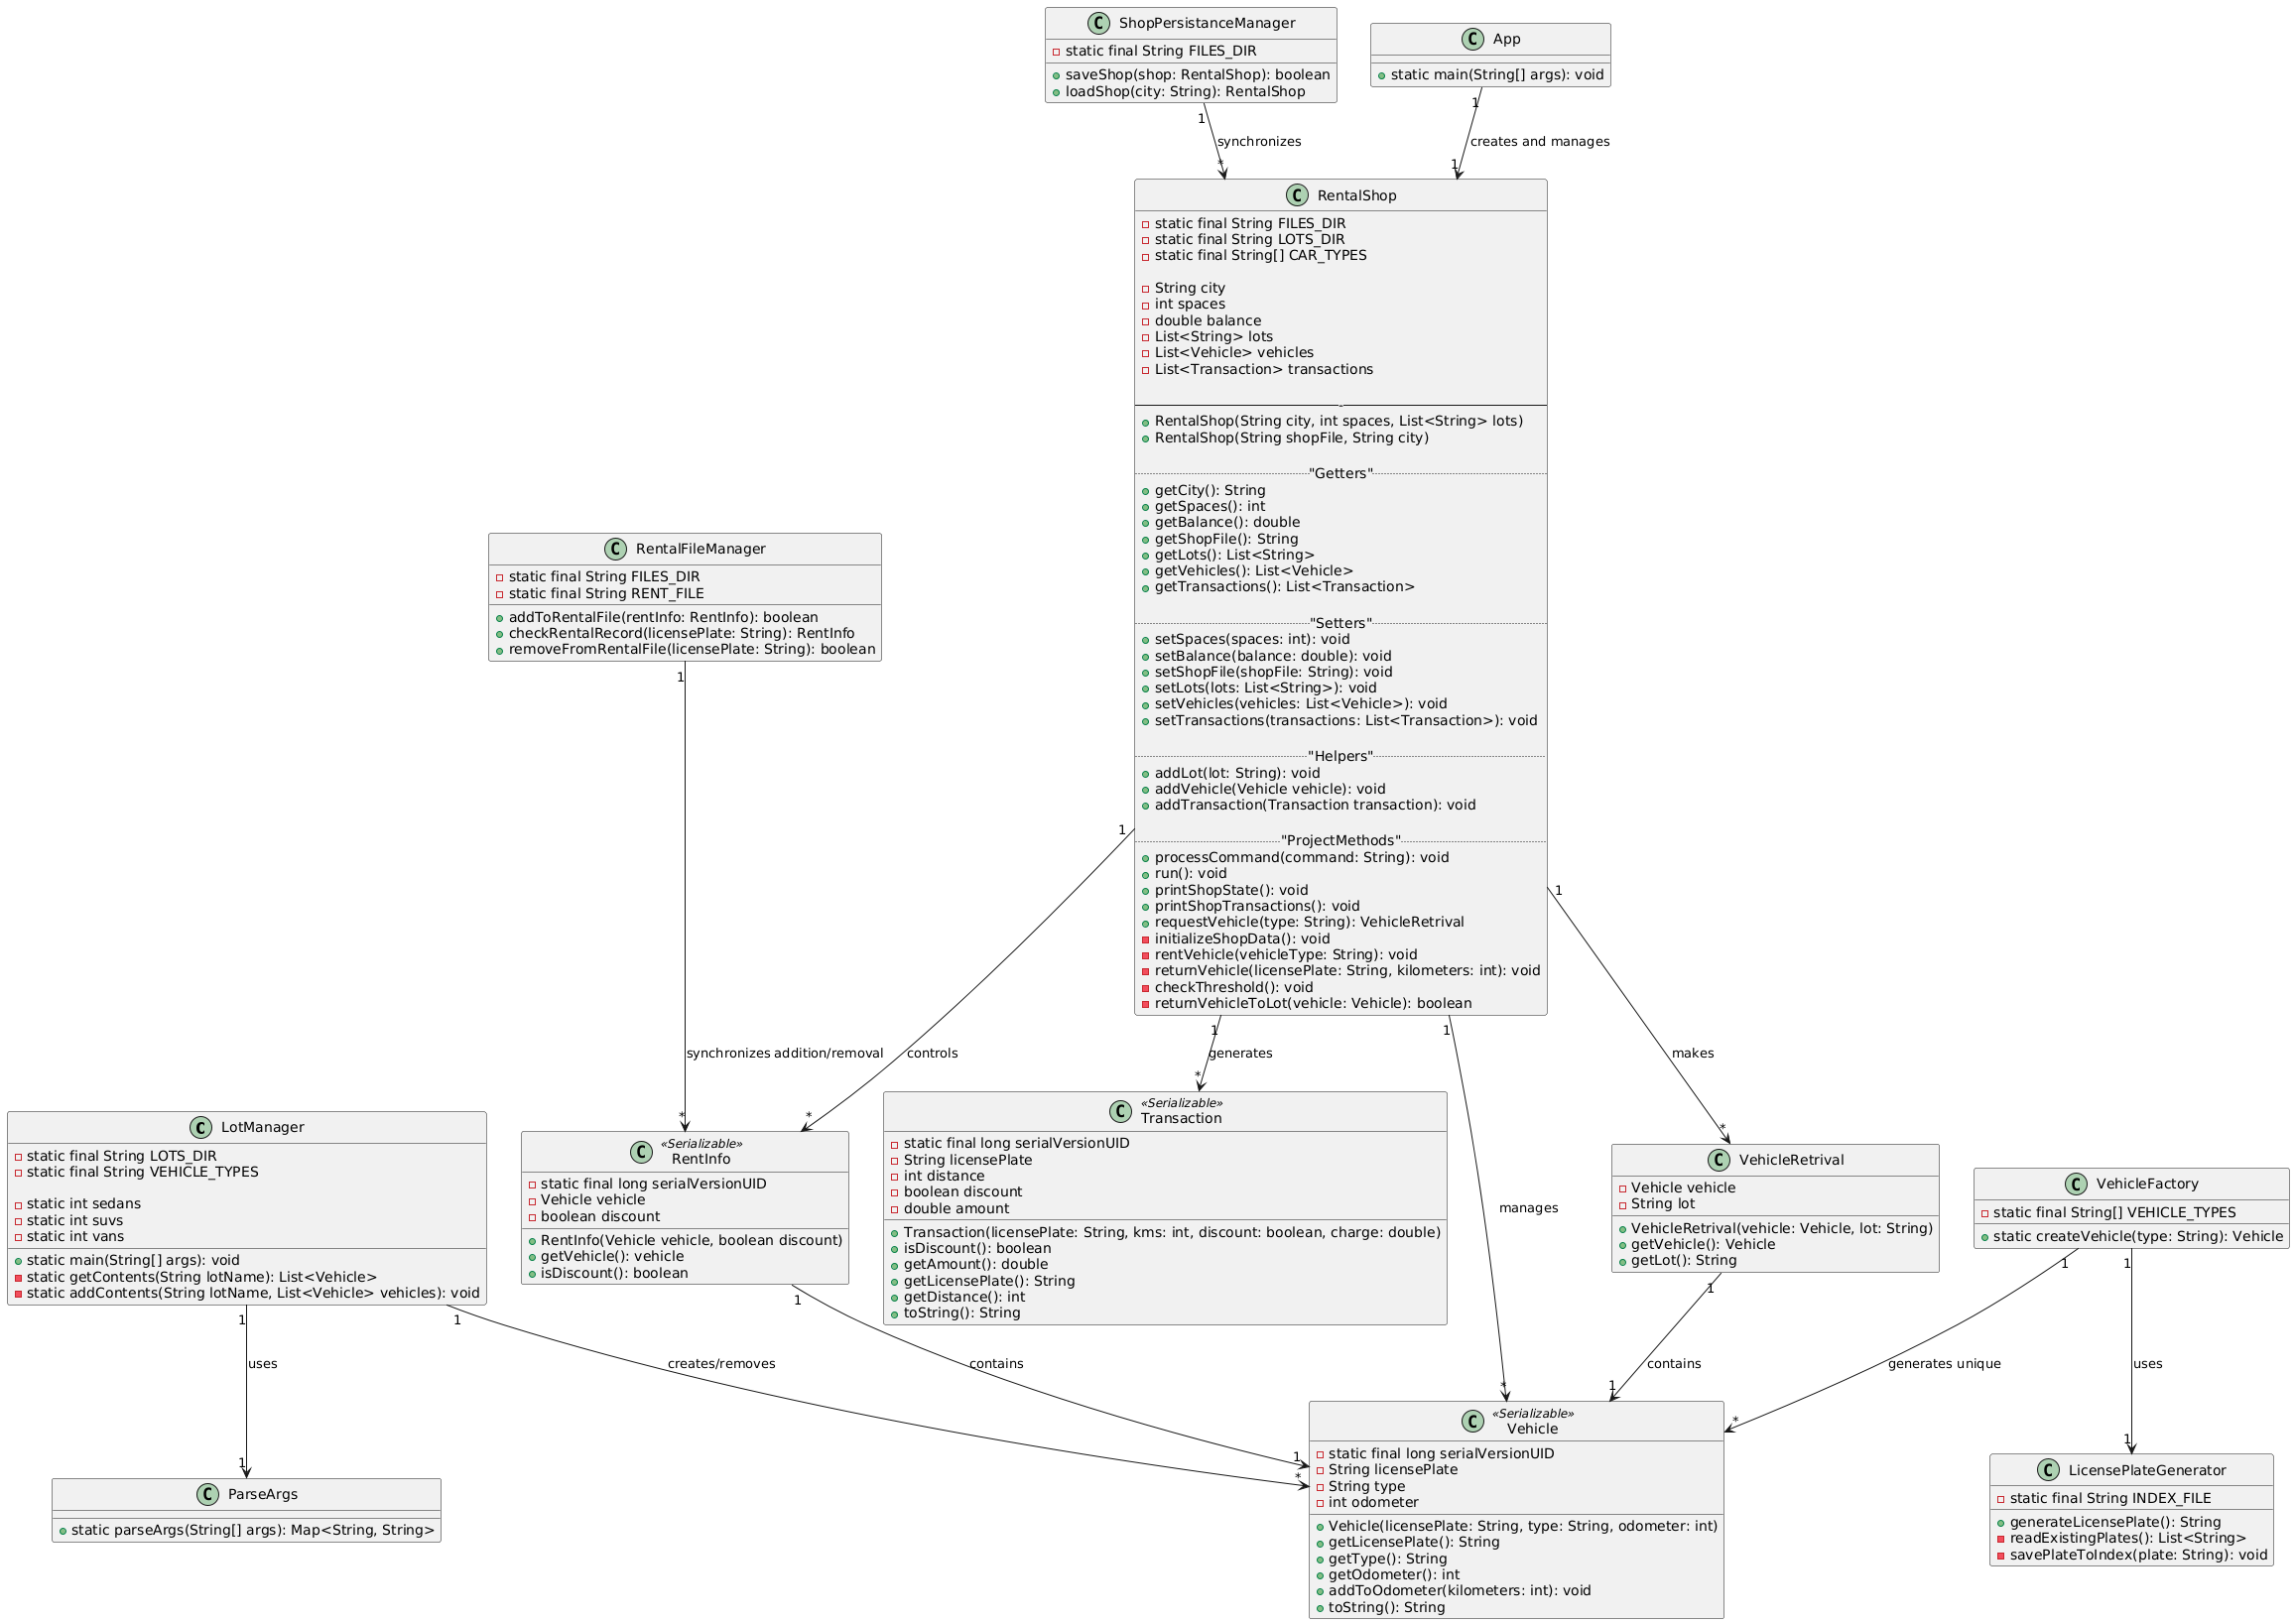
\includegraphics[width=\textwidth]{Diagram/ClassDiagram.png}
    \caption{\centering UML Diagram of the Car Rental System.}
    \label{fig:uml_diagram}
\end{figure*}

\subsection{System Components}
The system is composed of several components/classes, each with its own responsabilities. In this section, we will describe the main idea behind each of the classes in the system, and how they interact with each other. 

\subsubsection{LotManager Class}
The LotManager class is responsible for creating the lot, addition and deletion of vehicles. It is the main entry point for the whole system, since before creating a functional rental shop, the user must create a vehicle lot with some multiple vehicles. The class is responsible only for the creation of the lot, and the addition and removal of vehicles under the functionality specified in the project definition document. Communication with the rental shop is performed through the RentalShop class, which is responsible for managing the rental process. 

This class communicates with the VehicleFactory class to create randomized vehicles, with unique license plates. The class creates a file with the lot name in the ``lots'' directory, and initializes the lot with the specified number of vehicles with the use of flags. The class also implements the functionality to remove vehicles from the lot, and to add vehicles to the lot. 

\subsubsection{VehicleFactory Class}
The VehicleFactory class is responsible for creating vehicles with unique license plates. The class implements a factory method that creates a vehicle of the specified type (sedan, SUV, or truck) and assigns a unique license plate to the vehicle. The class interacts with the LicensePlateGenerator class to generate unique license plates for the vehicles. 

\subsubsection{LicensePlateGenerator Class}
The LicensePlateGenerator class is responsible for generating unique license plates for the vehicles. The class implements a simple algorithm that generates a random license plate with the format ``ABC-123'', where ``ABC'' is a random string of three uppercase letters and ``123'' is a random string of three digits. The class ensures that the generated license plates are unique by keeping track of the previously generated license plates, stored in the ``index.txt'' file, and checking if the generated license plate already exists in the file. 

\subsubsection{ParseArgs Class}
The ParseArgs class is responsible for parsing the command line arguments passed to the program. The class implements a simple parser that retrieves flags and their values from the command line arguments, and returns them in a map. This helps relieve the LotManager class and the RentalShop class from having to deal with the command line arguments directly. 

\subsubsection{RentalShop Class}
The RentalShop class is responsible for managing the rental process, including checking out and returning vehicles, and maintaining the shops state across multiple executions. This class is the second main entry point of the system, since it contains the business logic of the second part of the project. The class implements the core functionality of the rental shop system, including the ability to rent out and return vehicles, and to list the current state and transactions of the rental shop. 

The class utilizes with multiple classes to perform the required functionality. It retrieves vehicles found on the ``lot'' files by using the VehicleRetrival class, which is a simple Object that contains information about the vehicle and the lot it belongs to. The class communicates with the RentalFileManager class to keep track of the RentInfo object instances that are created whenever a vehicle is rented. The class also generates transactions whenever a vehicle is returned to the shop. 

The implementation tries to maximize the amount of money made by pre-initializing some vehicles in the rental shop whenever a new shop is created. The class will attempt to fill up the rental shop below $n-2$ spaces, where $n$ is the number of spaces available in the rental shop. This is done to ensure that the rental shop is always ready to rent out vehicles, and to minimize the amount of money lost to the $10\%$ discount that vehicles rented from lots have. 
Additionally, the class implements a simple algorithm to maintain the number of vehicles in the rental shop at an acceptable value, by checking if the number of vehicles is nearing the maximum number of vehicles allowed in the rental shop whenever a car is returned. If the number of vehicles is nearing the maximum number of vehicles allowed, the class will return some vehicles to the lots based on the mileage of each car. Low mileage vehicles are returned first, and the class will check if the vehicle is available in the lot before returning it. The class will also check if the vehicle is available in the rental shop before returning it.

Finally, this class manages to maintain the state of the rental shop across multiple parallel and separate executions by using save files in the ``shops'' directory. The ShopPersistanceManager class is utilized by the RentalShop class to save and load the state of the rental shop to and from the file. The class loads the state of the rental shop from the file whenever the user performs a command that needs to check the state of the rental shop; it saves the state of the rental shop whenever the program modifies the state of the rental shop. This ensures that the state of the rental shop is always up to date and consistent across multiple executions.

\subsubsection{RentalFileManager Class}
The RentalFileManager class is responsible for managing the rental file that contains the information about current rentals across all rental shops. The class implements a simple file manager that creates and manages the ``rentals'' file in the ``stores'' directory. The class is passed a RentInfo object whenever a vehicle is rented, and it will append the information to the ``rentals'' file. The class also implements a simple algorithm to check if a vehicle is already rented by checking if the license plate of the vehicle is already in the ``rentals'' file. The class is also responsible for removing the rental information from the ``rentals'' file whenever a vehicle is returned. 

\subsubsection{ShopPersistanceManager Class}
The ShopPersistanceManager class is responsible for managing the state of the rental shop across multiple executions. The class implements a simple file manager that creates and manages the RentalShop files in the ``shops'' directory. The class is passed a RentalShop object whenever the state of the rental shop needs to be saved, and it will save the state of the rental shop to the file. However, whenever it loads a rental shop it returns a temporary instance of the RentalShop class, by checking if a city with the same name already exists in the ``shops'' directory. The class will check if the file already exists, and if it does, it will load the state of the rental shop from the file and return it. 

\subsubsection{Other Classes}
The other classes in the project are simple data classes that are used to store and communicate information about vehicles, transactions, rental information, and retrivals; they don't implement any functionality but they are highly important for the system to work since they permit proper communication between the different components of the system.

\subsection{Files and Directories}
The system files and directories that contain the data of this project are organized all in the ``files'' directory, and separated into three directories: ``lots'', ``shops'', and ``indexes''. The ``lots'' directory contains the files that represent the vehicle lots, the ``stores'' directory contains the files that represent the rental shops, and the ``indexes'' directory containing the license plate index file. 

\subsubsection{Lots Directory}
The files in the ``lots'' directory are \textit{txt} files that contain the information about the vehicles in the lot. The files are named after the lot name, and they contain the vehicles currently in the lot. The format of the files is as follows:

\begin{lstlisting}[style=input]
<license_plate>,<vehicle_type>,<mileage>
<license_plate>,<vehicle_type>,<mileage>
...
\end{lstlisting}

Each line represents a vehicle in the lot, where the license plate is a string, the vehicle type is a string (either sedan, SUV, or truck), and the mileage is an integer. The files are created by the LotManager class whenever a lot is created, and they are updated whenever a vehicle is added or removed from the lot. The files are also used by the RentalShop class to retrieve and return vehicles from and to the lots.

\subsubsection{Shops Directory}
There are two types of files in the ``shops'' directory: the rental shop files and the rentals file. The rental shop files are \textit{txt} files that contain the information about the rental shops. The files are named after the rental shop name, and the entire state of the rental shop is saved in the file. The format of the files is as follows:

\begin{lstlisting}[style=input]
City:<city_name>
Spaces:<total_spaces>
Balance:<total_balance>
Lots:<lot1,lot2,...>
Vehicles:
<license_plate>,<vehicle_type>,<mileage>
<license_plate>,<vehicle_type>,<mileage>
... 
Transactions:
TRANSACTION: <license_plate>; Distance: <distance> km; Discount: 0% || 10%; Amount: $<amount>
TRANSACTION: <license_plate>; Distance: <distance> km; Discount: 0% || 10%; Amount: $<amount>
...
\end{lstlisting}

The files contain all the information about the rental shop, including the city name, total spaces, balance, lots, vehicles, and transactions. This information is used by the RentalShop class and the ShopPersistanceManager class to manage the state of the rental shop across multiples executions. The rentals file is a \textit{txt} file that contains the information about the current rentals across all rental shops, without this file cars wouldn't be able to be returned to any rental shop. The file is named ``rentals.txt'', and it contains the information about the current rentals. The format of the file is as follows:

\begin{lstlisting}[style=input]
<license_plate>,<vehicle_type>,<mileage>,<discount> 
<license_plate>,<vehicle_type>,<mileage>,<discount>
... 
\end{lstlisting}

The file contains the information about the current rentals, where the license plate is a string, the vehicle type is a string (either sedan, SUV, or truck), the mileage is an integer, and the discount is a boolean; represents whether a discount applies. The file is created and maintained by the RentalFileManager class whenever a vehicle is rented, and it is updated whenever a vehicle is returned.

\subsubsection{Indexes Directory}
Lastly, the ``indexes'' directory contains the license plate index file. The file is named ``index.txt'', and it contains the information about the license plates that have been generated by the LicensePlateGenerator class. The contents of the file are simply one license plate per line, and it is used to ensure that the generated license plates are unique. The file is created and maintained by the LicensePlateGenerator class whenever a new license plate is generated.


\subsection{Testing}
The project was tested using a System Testing approach, where the system was tested as a whole. The reason for this approach is because the project is heavily dependent on the interaction between the different components of the system, and the behavior they enforce on the file system. There are two tests the user can run, one for the LotManager class and another for the RentalShop class. The tests are located in the ``tests'' directory, and they are named ``LotManagerTest.java'' and ``RentalShopTest.java''. The tests are implemented using the JUnit testing framework, and they can be run through the Script provided in the ``Car\_Rental'' directory. The tests are designed to test the functionality of the LotManager class and the RentalShop class, and they cover the main functionality of the system. The tests are not exhaustive, but they cover the main functionality of the system and ensure that the system works as expected.

The tests are designed to be run in a clean environment, where the ``lots'', ``shops'', and ``indexes'' directories are empty. The tests will create the necessary files and directories, and they will clean up after themselves by deleting the files and directories created during the tests. The tests will also check if the files and directories were created successfully, and if the contents of the files are as expected. The tests will also check if the system behaves as expected when the user performs different actions, such as creating a lot, adding vehicles, renting vehicles, returning vehicles, and listing the state of the rental shop.

Manual testing was also performed to ensure that the system worked as expected under the following scenarios: 
\begin{itemize}
    \item Creating a lot with multiple vehicles and checking if the vehicles were created successfully.
    \item Creating a rental shop with multiple lots and checking if the rental shop was created successfully.
    \item Renting a vehicle from the rental shop and checking if the vehicle was rented successfully.
    \item Returning a vehicle to the rental shop and checking if the vehicle was returned successfully.
    \item Returning a vehicle to another rental shop and checking if the vehicle was returned successfully.
    \item Listing the state of the rental shop and checking if the state was listed successfully.
    \item Checking if the rental shop was able to return vehicles to the lots when the space was exceeded.
    \item Checking if various rental shop executions were able to maintain the state of the rental shop across.
\end{itemize}

The tests are showcased in a YouTube video developed by the author, which can be found at the following link: \href{https://youtu.be/x1P02jSwtFk}{Extra Tests}. The video showcases the functionality of the system, and it demonstrates how to use the system. The video also showcases the tests that were performed on the system, and it demonstrates how to run the tests.

\section{AI Disclosure}
The project was developed with the help of GitHub copilot, which is an AI-powered code completion tool. The tool was used to help generate the test files and the class diagram, as well as to help understand the concepts of file locking in the Java programming language. The rest of the project was developed by the author. 

The reason for the use of AI tools was to help speed up the development process and to help understand certain concepts that were not clear from the documentation provided by Oracle; primarily the file locking concepts. Note, the file management in this project was performed entirely by the author; the AI tool helped me understand how it worked but the development was performed by the author. 

Lastly, the tests were primarily generated by the AI tool since the author had already tested the functionality of the system manually but due to the heavy usage of file management, the AI tool facilitated the process of creating the tests. 

\section{Conclusion}
Throughout the development of this project, we have explored the principles of memory management and file system controls. We have implemented a Car Rental System that demonstrates how to manage memory effectively, providing process synchronization, data integrity, and resource tracking. The project has also showcased how applications interact with the underlying operating system to maintain state across executions. 

The deliverables of this project demonstrate the correct functionality of the system, and the tests provided ensure that the system works as expected. 
\end{document}